% !TeX encoding = windows-1251
\documentclass[fullscreen=true,russian,compress,%
	hyperref={unicode,bookmarks=false}]{presentation}
\inputencoding{utf8} % Кодировка вашего файла
% Внимание! Опция russian не совместима с \tableofcontents
\usepackage[russian]{babel} % Эту строку можно удалить
\usepackage{paratype} % Выбираем шрифт
% Определяем длины частей нижнего колонтитула: автор, название, число слайдов
\makefootline{.35}{.55}{.1} % Сумма длин = 1

\usepackage{tikz} % Для создания рисунков с помощью tikz
\usepackage{listings} % Для листингов программ

\begin{document}

% Если потребуется, переводим названия блоков с английского:
\deftranslation[to=Russian]{Theorem}{Теорема}
\deftranslation[to=Russian]{Example}{Пример}

% Данные титульного слайда
\title[Разработка инструмента экспорта данных моделей в формате XML]{Разработка инструмента экспорта данных моделей в формате XML}
\author{Лавров Михаил Андреевич}
\institute{Научный руководитель: И.\,В.~Парамонов}
\date{24.06.2023}

% Создаем титульный слайд
\begin{frame}
\titlepage
\end{frame}

% \tableofcontents не работает при включенной опции russian пакета babel
%\begin{frame}{Содержание}\tableofcontents\end{frame}

\section{Ведение}

\begin{frame}{Введение}

\begin{block}{Описание проекта}
    Задача была реализована в рамках проекта АСП ФК (Автоматизированная система планирования Федерального Казначейства). Основные его предназначения -- планировать, назначать и проводить проверки организаций. Также он позволяет взаимодействовать подразделениям Казначейства между собой.
\end{block}

\begin{block}{Актуальность задачи}
    Потребность в реализации такого инструмента в проекте возникла из--за необходимости интеграции с системой ЕРП (Единый реестр проверок). Данной системе было необходимо предоставить информацию о планах Казначейства.
\end{block}

\end{frame}

\begin{frame}{Применимость существующих инструментов}

\begin{block}{Применимость существующих инструментов}
    Существующие инструменты (JAXB, Jackson, XStream и д.р.) не подходят, так как для реализации всех пунктов постановки придётся использовать аннотации, что не соответствует требованиям постановки, а также неудобно, так как кроме работы с интерфейсом приходится работать и с кодом проекта.
\end{block}

\end{frame}

\section{Описание задачи}

\begin{frame}{Постановка задачи}

Необходимо разработать инструмент экспорта данных моделей и создать интерфейс для его использования.

    \begin{block}{Главные пункты в постановке к задаче}
        \begin{enumerate}
	      \item Необходима возможность взаимодействия с инструментом с помощью интерфейса в проекте.
	      \item Если нужно создать новую схему экспорта, то модель, описанная в Java--интерфейсе, не должна быть затронута.
	      \item Нужна поддержка добавления тегов с фиксированным значением, вложенных в корневой элемент.
        \end{enumerate}
    \end{block}
    
\end{frame}

\section{Основная часть}

\begin{frame}{Описание нужной структуры}

Для демонстрации работы инструмента будет создана следующая структура экспорта.

\centerline{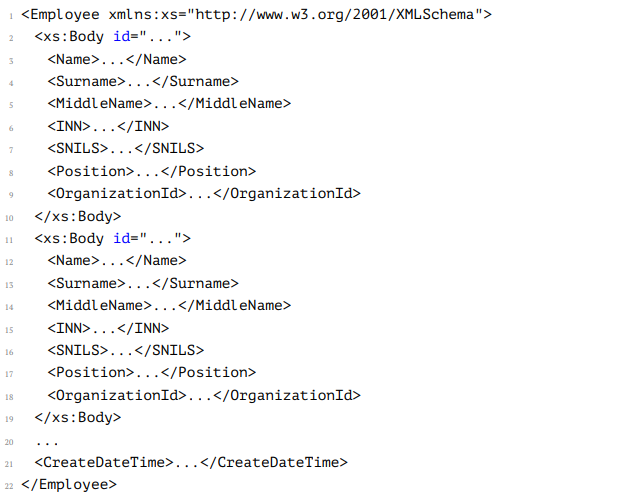
\includegraphics[width=0.7\textwidth]{imgs/xmlexampleasimg.png}}

\end{frame}

\begin{frame}{Создание источника данных}

Для начала необходимо создать аналитический источник данных в соответствующем интерфейсе.
\hfill
\centerline{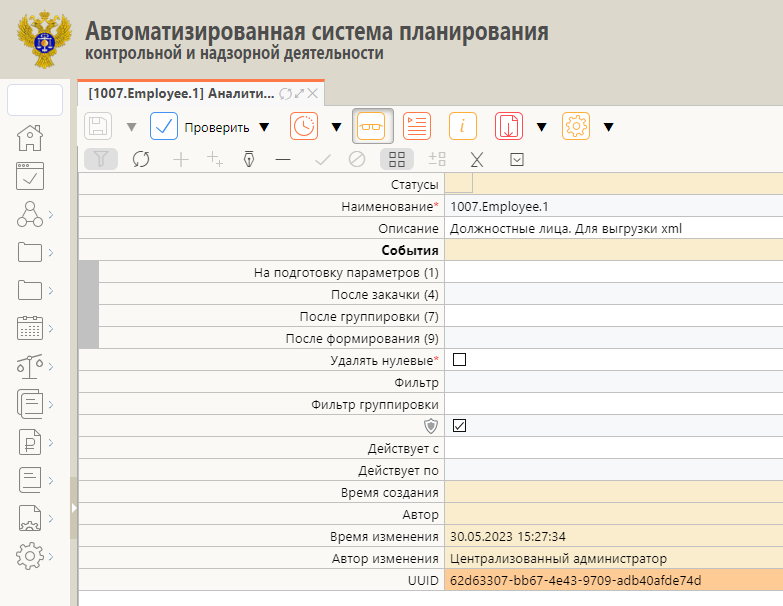
\includegraphics[width=0.8\textwidth]{imgs/source.png}}

\end{frame}

\begin{frame}{Создание новой структуры экспорта}

Далее создаётся запись в интерфейсе <<Структура экспорта xml>>, в которой указывается созданный источник данных.
\hfill
\centerline{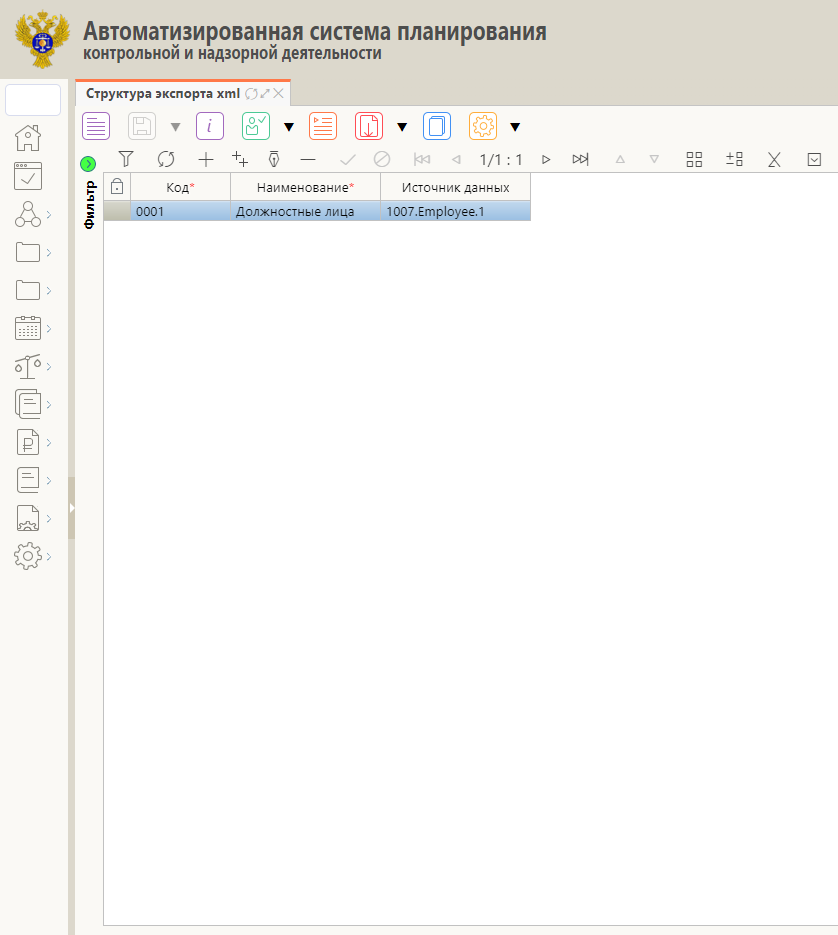
\includegraphics[width=0.8\textwidth]{imgs/main.png}}

\end{frame}

\begin{frame}{Создание пространства имён}

Для структуры экспорта задаются пространства имён, которые будут использованы тегами.
\hfill
\centerline{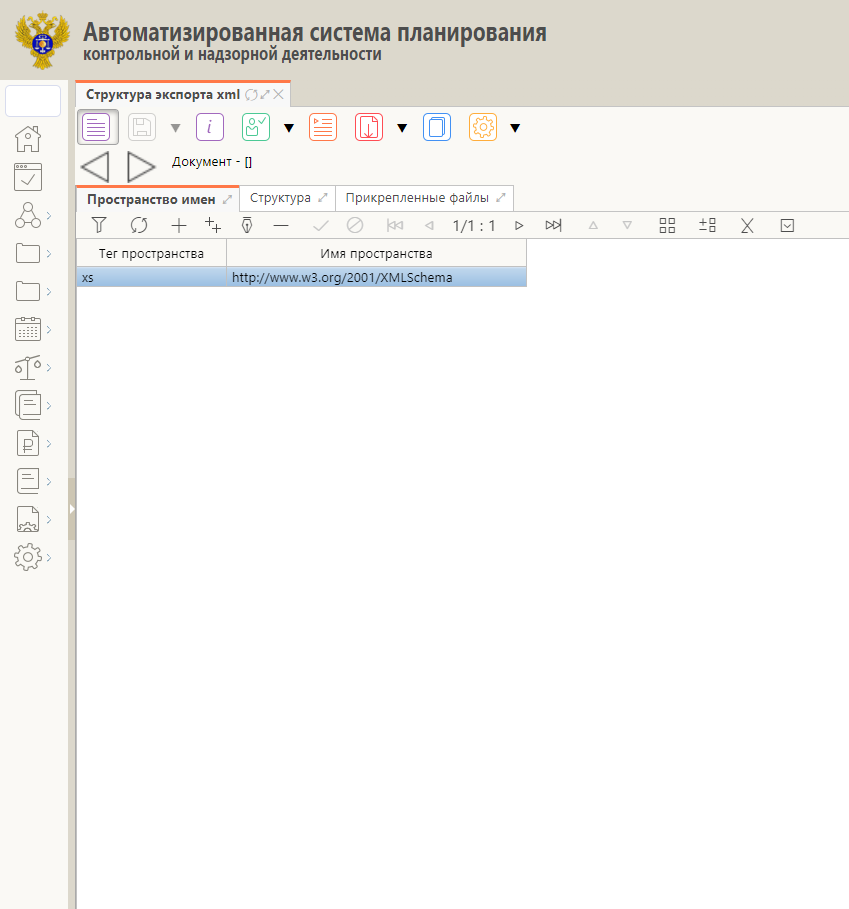
\includegraphics[width=0.8\textwidth]{imgs/Namespaces.png}}

\end{frame}

\begin{frame}{Создание структуры элементов}

Далее необходимо создать запись для каждого тега и прописать в соответствующих колонках нужные значения.
\hfill
\centerline{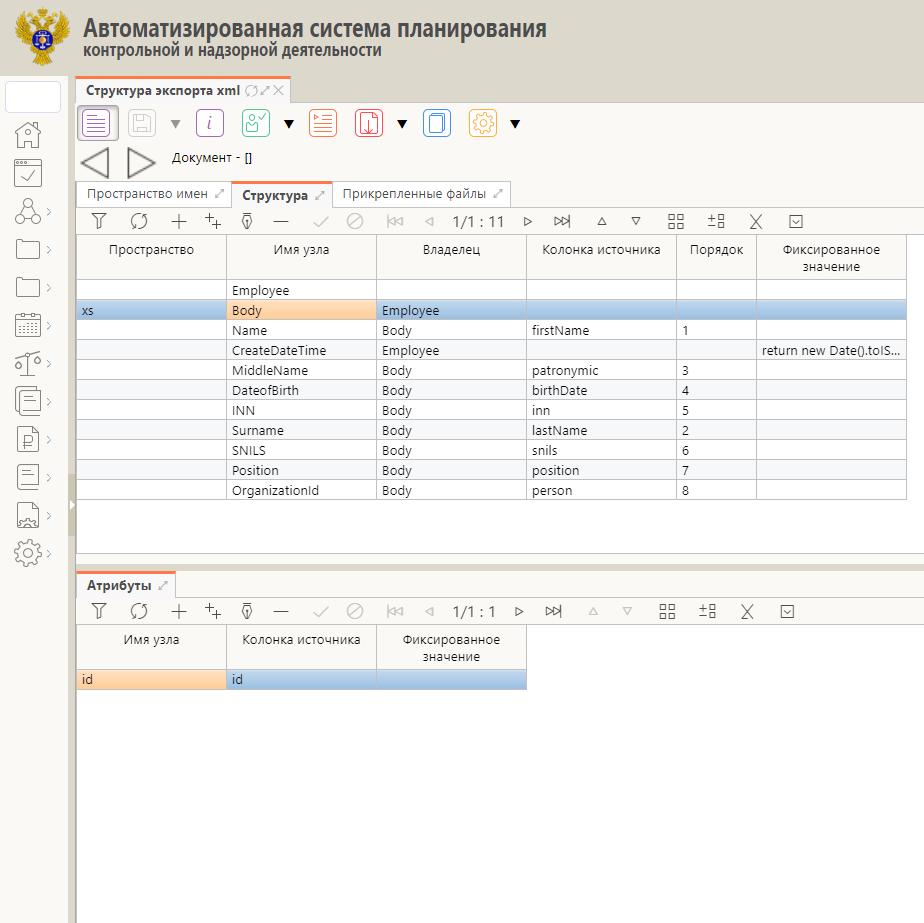
\includegraphics[width=0.8\textwidth]{imgs/struct.png}}

\end{frame}

\begin{frame}{Результат генерации}

Далее, при тестовой генерации, получается такой документ (представлен в обезличенном виде).
\hfill
\centerline{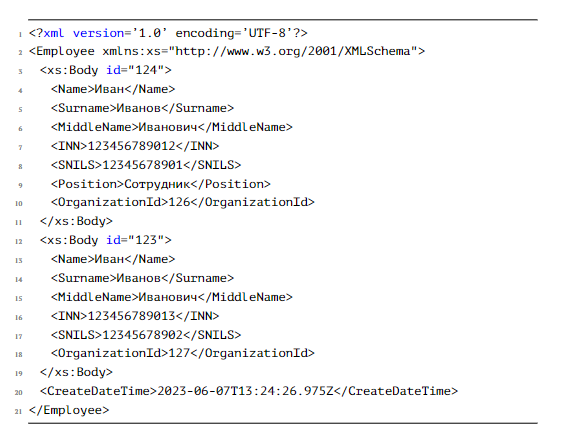
\includegraphics[width=0.7\textwidth]{imgs/generatedexmaple.png}}
    
\end{frame}

\begin{frame}{Используемая технология}

XML-документ будет генерироваться по принципу StAX. Его главное преимущество перед подходом DOM -- это возможность записи данных последовательно, без необходимости генерации заранее структуры элементов, которая необходима в DOM. 
\hfill
\centerline{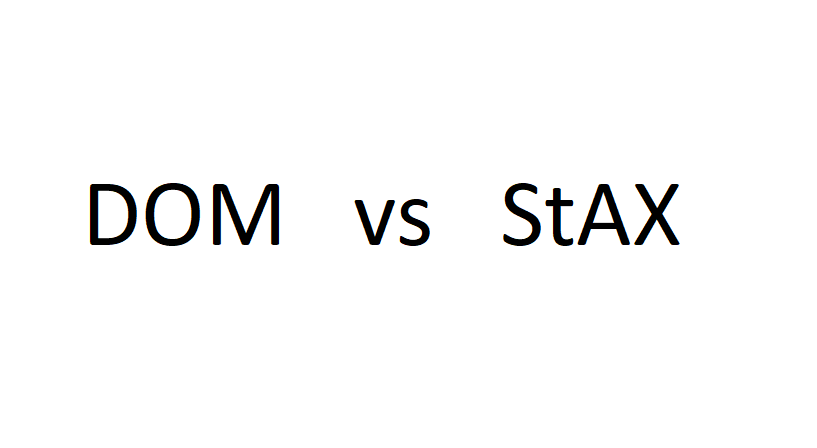
\includegraphics[width=0.8\textwidth]{imgs/staxvsdom.png}}
\end{frame}

\section{Описание способа взаимодействия с инструментом}

\begin{frame}{Взаимодействие с помощью сервлета}

Взаимодействие происходит с помощью сервлета. Ниже представлена диаграмма последовательности для GET-запроса.

\hfill

\centerline{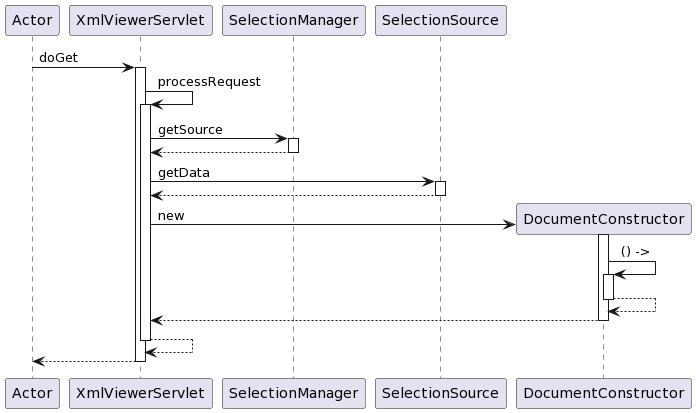
\includegraphics[width=0.7\textwidth]{imgs/usingservlet.png}}

\end{frame}

\section{Описание алгоритма генерации}

\begin{frame}{Описания принципа генерации документа по структуре}

\centerline{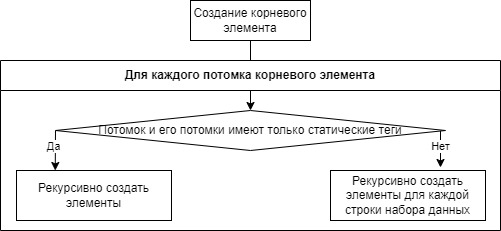
\includegraphics[width=\textwidth]{imgs/diagr.jpg}}

\end{frame}

\begin{frame}{Результат разработки}

В результате получились:

\begin{enumerate}
	\item[4] класса, описывающие модели данных
    \item[1] класс, отвечающий за работу сервлета
    \item[1] класс, отвечающий за создание документа
    \item[12] методов, отвечающих за создание документа
    \item[870] строк кода
\end{enumerate}

\end{frame}

\section{Заключение}

\begin{frame}{Заключение}
     \begin{block}{В результате работы были разработаны}
        \begin{enumerate}
	      \item Интерфейс в проекте, позволяющий создавать структуру тегов в документе.
            \item Инструмент, позволяющий по структуре и набору данных создавать XML-документ.
            \item Инструмент был протестирован, его работа была сверена с постановкой отделом тестирования ООО <<НПО <<Криста>> и он был внедрён в проект АСП ФК.
        \end{enumerate}
    \end{block}
\end{frame}

\appendix

\end{document}
